% !TEX root = ../main.tex
\section{Introduction}

Deep research agents turn a question into an investigation. A supervisor first decomposes the question into sub-tasks and dispatches them to several researchers. Each researcher searches the web, reads sources, and writes a \emph{summary}. The supervisor reflects on the returned summaries and may launch further rounds of research. A writer finally reads all summaries and produces a long, citation-grounded \emph{report}. Every role issues one or even more LLM calls. In this pipeline the bottleneck is LLM inference, not retrieval: on the workload we study, the LLM calls take about 92\% of end-to-end wall-clock time. We study this workload at the LLM-call layer, over a trace of 800 tasks and 15,296 generation calls, and find a defining property: \textbf{content recycling}. A span of text is generated once, yet the pipeline serves it many times. This recycling appears on both sides of inference. During prefill, the same content is re-read by later calls, so its KV cache is recomputed from scratch again and again. During decode, the content is re-generated---copied, often verbatim, into later outputs. To our knowledge, this is the first content-level characterization of deep research inference; prior agent traces stop at the systems level and discard the text~\cite{tracelab}. \emph{Once generated, many times served.}

Recycling is easy to name but hard to collect, because the workload is heterogeneous while existing techniques are uniform. On the prefill side, cross-request KV reuse skips recomputation by blending a cached KV into the new prompt~\cite{cacheblend,kvcomm,droidspeak}. But the blended KV is only approximate. Blending it blindly shifts what a downstream agent attends to, which changes the agent's decisions and degrades report quality. Prior methods choose which tokens to recompute by KV deviation alone~\cite{cacheblend}; yet a token whose KV deviates greatly but that no downstream query attends to does not affect the output. On the decode side, suffix-based speculation drafts the next tokens directly from repeated content~\cite{suffixdecoding}, but it runs the same way on every call. Copy rates vary widely: some calls copy their input almost verbatim, others rewrite and condense it (8--91\%, bimodal). A single fixed drafter therefore wins on copy-heavy calls but loses on rewrite-heavy ones. Prior methods adapt the drafter \emph{during} a call, tuning draft length from the drafts accepted so far~\cite{specdecpp,banditspec}. None routes on a call's copy rate---the property that decides which drafter fits---which our characterization shows is predictable \emph{before} the call begins.


\begin{figure}[t]
    \centering
    \resizebox{0.95\linewidth}{!}{
    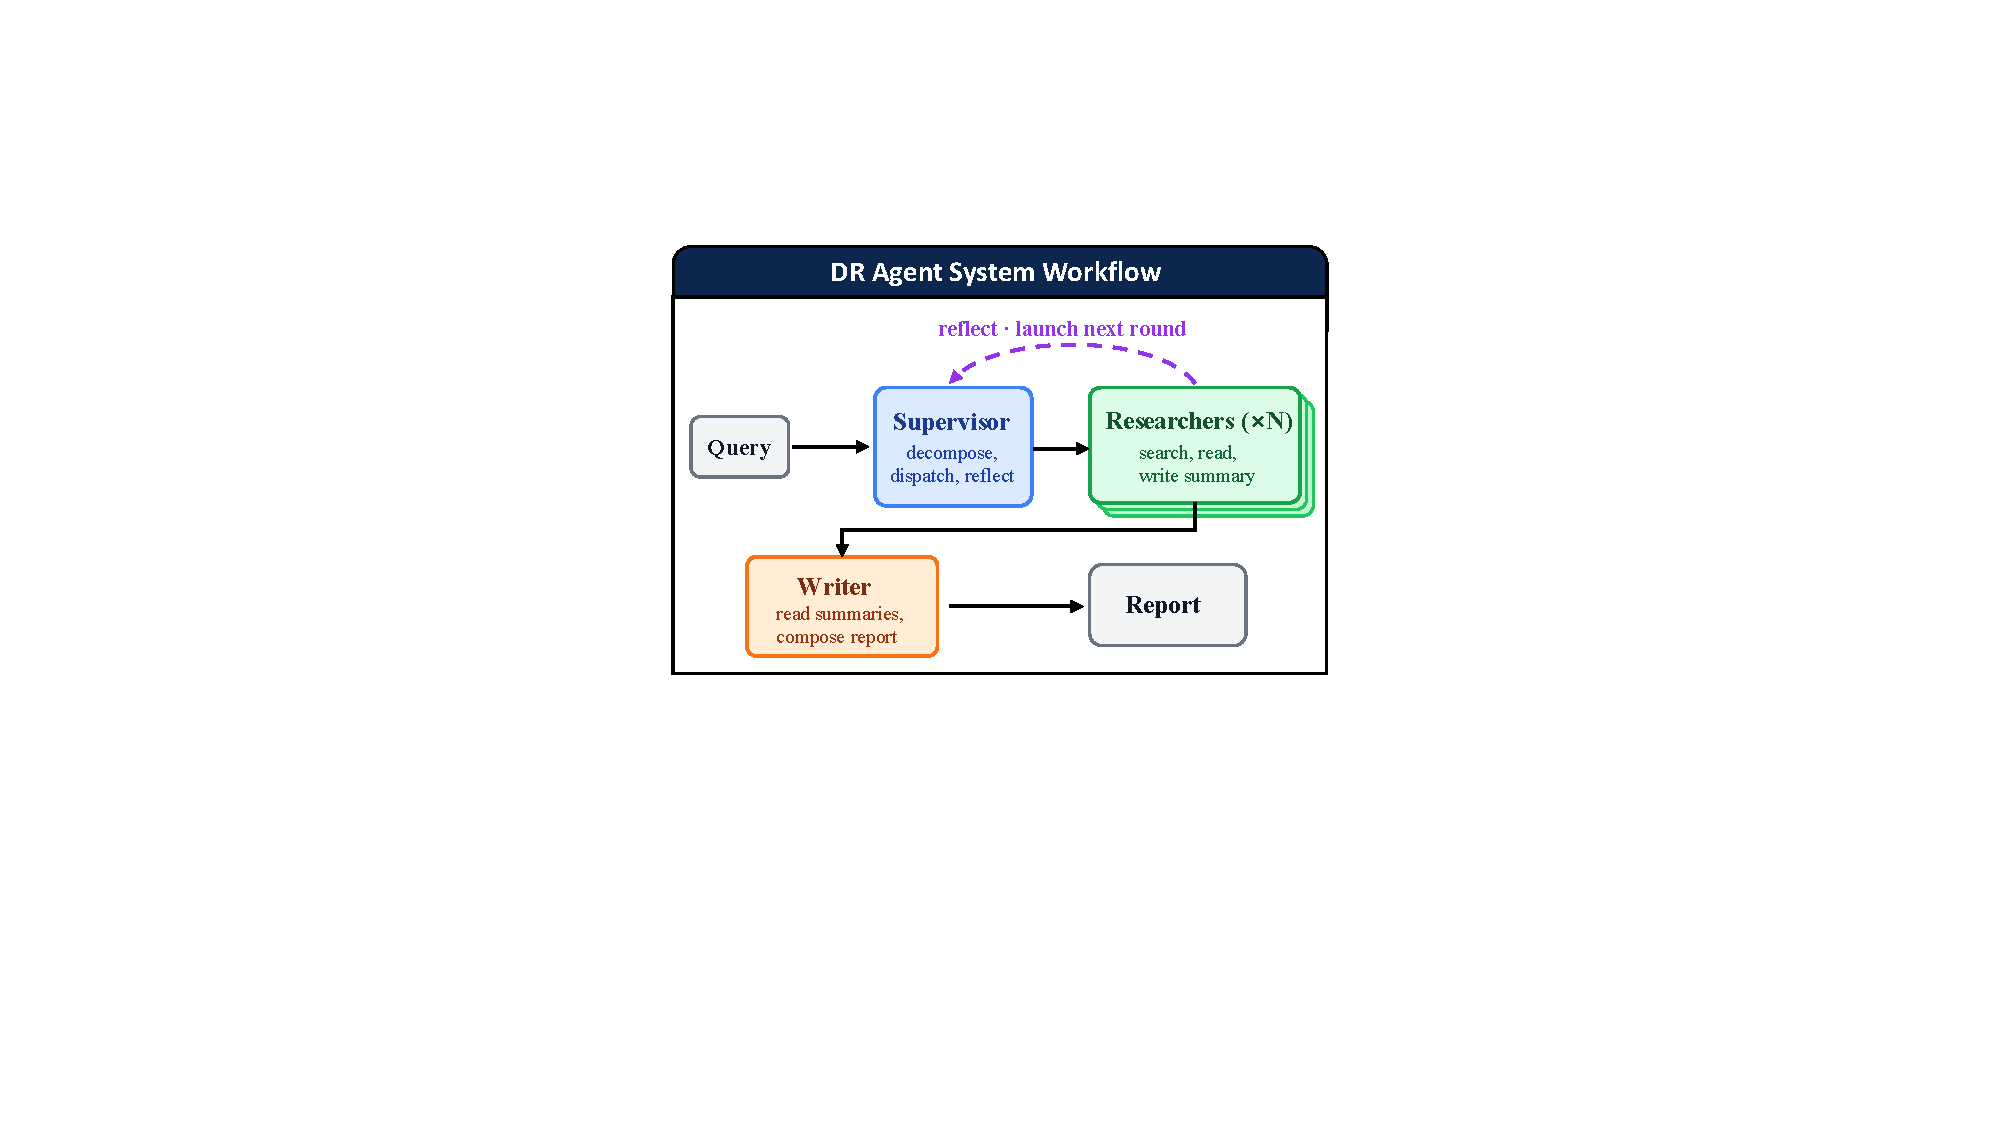
\includegraphics[trim=32em 20em 32em 10em,clip,width=1\linewidth]{Figures/workflow.pdf}
    }
    \caption{
    The deep research agent workflow. A supervisor decomposes the query and dispatches sub-tasks to parallel researchers; each researcher searches, reads, and writes a summary; the supervisor reflects and may launch further rounds; a writer composes the final report.
    }
    \label{fig::overview}
\end{figure}

We exploit recycling on both sides, and we match the mechanism to each call. On the prefill side, we propose \emph{attention-guided selective recomputation}: we recompute a reused token only when its KV deviation is large \emph{and} the downstream query attends to it heavily; a token that deviates greatly but draws little attention is reused unchanged. On the decode side, we route speculative decoding by predicted copy rate: a lightweight predictor reads the target model's hidden state and, under a simple cost model, selects both the drafter and the draft depth, so that each call runs its most economical strategy. For rewrite-heavy calls, where little text can be copied, off-the-shelf draft heads fail on this workload; we therefore train an EAGLE-3 draft head on the agent's own trajectories. We train both the copy-rate predictor and the specialized head. On mainstream deep research benchmarks, our system cuts end-to-end latency by up to 56.3\% versus vLLM, with report quality statistically unchanged. This paper makes four contributions:

\begin{itemize}
\item \textbf{Characterization.} We present the first content-level characterization of deep research inference at the LLM-call layer, and show that content is recycled on both the prefill and the decode side, in amounts that vary sharply across calls.
\item \textbf{Attention-guided selective recomputation.} On the prefill side, we recompute a reused token only when its KV deviation and its downstream attention are \emph{both} high, avoiding both the quality loss of blind blending and the wasted work of deviation-only selection.
\item \textbf{Copy-rate-routed speculative decoding.} On the decode side, a hidden-state predictor selects the drafter and the draft depth per call under a cost model; for rewrite-heavy calls we add an EAGLE-3 head specialized on the agent's own trajectories.
\item \textbf{System and evaluation.} We integrate both sides and evaluate end-to-end on deep research benchmarks, cutting latency by up to 56.3\% with statistically unchanged report quality.
\end{itemize}
